\documentclass[11pt,a4paper]{article}

\usepackage[utf8]{inputenc}
\usepackage[T1]{fontenc}
\usepackage[spanish]{babel}
\usepackage{geometry}
\usepackage{graphicx}
\usepackage{array}
\usepackage{tabularx}
\usepackage{makecell}
\usepackage[table]{xcolor}
\usepackage{fancyhdr}
\usepackage{titlesec}
\usepackage{helvet}
\usepackage{ragged2e}
\usepackage{enumitem}
\usepackage{setspace}
\usepackage{hyperref}
\usepackage{booktabs} % Para tablas con acabado profesional
\usepackage{alltt}    % Bloque monoespaciado que si admite macros (lambda, mu, rho)
\usepackage{amsmath}  % Para las formulas del modelo

\renewcommand{\familydefault}{\sfdefault}
\geometry{
  a4paper,
  left=3.0cm,
  right=3.0cm,
  top=2.35cm,
  bottom=2.35cm,
  headheight=1.9cm,
  headsep=0.45cm
}

\setlength{\parindent}{0pt}
\setlength{\parskip}{0.22em}
\setlength{\emergencystretch}{2em}   % evita desbordes de linea en texto justificado
\setlength{\tabcolsep}{6pt}
\renewcommand{\arraystretch}{1.08}

\pagestyle{fancy}
\fancyhf{}
\fancyhead[L]{
\includegraphics[height=1.35cm]{assets/reporte_tecnico_overleaf_logo.png}}
\fancyhead[R]{\vspace{0.1cm}\small FEIRNNR - Carrera de Computación}
\renewcommand{\headrulewidth}{0.5pt}
\renewcommand{\footrulewidth}{0pt}
\makeatletter
\renewcommand{\headrule}{%
  {\color{gray!65}\hrule width\headwidth height\headrulewidth \vskip-\headrulewidth}%
}
\makeatother

\titleformat{\section}
  {\bfseries\fontsize{15}{17}\selectfont}
  {\thesection.}{0.8em}{}
\titlespacing*{\section}{0pt}{0.7ex}{0.2ex}

\newcolumntype{L}[1]{>{\RaggedRight\arraybackslash}p{#1}}
\newcolumntype{Y}{>{\RaggedRight\arraybackslash}X}

% Marca visible de lo que el equipo todavia debe escribir.
\newcommand{\pendiente}[1]{\textcolor{red}{\textbf{[PENDIENTE: #1]}}}

% Paleta de las tablas de la plantilla institucional.
\definecolor{headerblue}{RGB}{19, 93, 126}
\definecolor{rowlight}{RGB}{205, 235, 248}
\definecolor{borderblue}{RGB}{64, 160, 206}

% babel-espanol renombra \tablename como "Cuadro"; el texto usa "Tabla".
\addto\captionsspanish{\renewcommand{\tablename}{Tabla}}

\begin{document}
\thispagestyle{fancy}

\vspace*{0.15cm}

\begin{center}
{\bfseries\fontsize{23}{26}\selectfont
Reporte Técnico de Actividades\\
Práctico-Experimentales Nro. 003\par}
\end{center}

\section{Datos de Identificación del Estudiante y la Práctica}

\noindent
\begin{tabularx}{\textwidth}{|L{0.43\textwidth}|Y|}
\hline
\textbf{Nombre del estudiante(s)} & Jaime Landázuri, Richard Chamba, Cael Soto, Domenica Rojas \\ \hline
\textbf{Asignatura} & Simulación \\ \hline
\textbf{Ciclo} & 5 A \\ \hline
\textbf{Unidad} & 1 \\ \hline
\textbf{Resultado de aprendizaje de la unidad} & R1. Aplica análisis estadísticos de los datos
de la Simulación para mejorar la calidad de los resultados, bajo los principios de solidaridad, transparencia, responsabilidad y honestidad. \\ \hline
\textbf{Práctica Nro.} & 003 \\ \hline
\textbf{Título de la Práctica} & Simulación de un sistema de líneas de espera M/M/1 mediante SimPy \\ \hline
\textbf{Nombre del Docente} & José O. Guamán Q. \\ \hline
\textbf{Fecha} & 15 de Octubre de 2026 \\
 & 16 de Octubre 2026 \\ \hline
\textbf{Horario} & Jueves 10h30 a 11h30 \\
 & Viernes 07h30 a 09h30 \\ \hline
\textbf{Lugar} & Aula \\ \hline
\textbf{Tiempo planificado en el Sílabo} & 3 horas \\ \hline
\end{tabularx}

\section{Objetivo(s) de la Práctica}
Simular un sistema de líneas de espera M/M/1 utilizando Python y SimPy, analizando
el comportamiento de los clientes, la cola y el servidor.
\begin{enumerate}
    \item Implementar un modelo M/M/1 utilizando la biblioteca SimPy.
    \item Calcular las principales métricas teóricas del sistema de espera.
    \item Comparar los resultados teóricos con los obtenidos mediante la simulación.
\end{enumerate}

\section{Materiales y reactivos}
\begin{itemize}
    \item Python 3.x (se ejecutó con Python 3.14.8).
    \item Biblioteca SimPy (se ejecutó con SimPy 4.1.2).
    \item NumPy (2.5.4).
    \item Matplotlib (3.11.2).
    \item Editor de código: Visual Studio Code, PyCharm o Jupyter Notebook.
\end{itemize}

\section{Equipos y herramientas}
\begin{itemize}
    \item Computador.
    \item Procesador de 2 núcleos o superior.
    \item Mínimo 4 GB de RAM.
    \item Sistema operativo Linux o macOS.
\end{itemize}

\section{Procedimiento / Metodología Ejecutada}

\subsection{Fundamento teórico}

El modelo \textbf{M/M/1} representa un sistema de líneas de espera con llegadas de
clientes siguiendo una distribución de Poisson, tiempos de servicio con distribución
exponencial, un único servidor y atención de clientes bajo el principio FIFO
(\emph{primero en llegar, primero en ser atendido}).

El modelo utiliza dos parámetros principales:
\begin{itemize}
    \item $\lambda$: tasa promedio de llegada de clientes.
    \item $\mu$: tasa promedio de servicio del servidor.
\end{itemize}

La utilización del servidor se calcula mediante:
\[
\rho = \frac{\lambda}{\mu}
\]

\noindent\textbf{Observación sobre la guía.} La guía de la práctica (§5.1) imprime
$\rho = \mu/\lambda$, lo que contradice su propia condición de estabilidad
$\lambda < \mu$ enunciada unas líneas más abajo y también su pseudocódigo, que usa
$\rho = \lambda/\mu$. Con la fórmula impresa, los tres escenarios de la guía darían
$\rho = 1{,}50$, $1{,}20$ y $1{,}03$, es decir un servidor saturado en los tres casos, y
las medidas $L$, $L_q$, $W$ y $W_q$ no existirían, porque solo están definidas para
$\rho < 1$. Este trabajo usa la definición correcta $\rho = \lambda/\mu$, que es la que
emplea el pseudocódigo de la propia guía y la que aparece en la bibliografía de teoría
de colas.

Para que el sistema sea estable debe cumplirse:
\[
\lambda < \mu
\]

Las principales medidas teóricas del sistema son:

\[
L = \frac{\lambda}{\mu-\lambda} \qquad
L_q = \frac{\lambda^2}{\mu(\mu-\lambda)}
\]

\[
W = \frac{1}{\mu-\lambda} \qquad
W_q = \frac{\lambda}{\mu(\mu-\lambda)}
\]

\begin{table}[h!]
\centering
\setlength{\arrayrulewidth}{0.75pt}
\arrayrulecolor{borderblue}
\renewcommand{\arraystretch}{1.25}
\begin{tabular}{|l|l|}
\hline
\rowcolor{headerblue}
\textbf{\textcolor{white}{Símbolo}} & \textbf{\textcolor{white}{Significado}} \\ \hline
$\lambda$ & Tasa de llegada de clientes \\ \hline
\rowcolor{rowlight}
$\mu$ & Tasa de servicio \\ \hline
$\rho$ & Utilización del servidor \\ \hline
\rowcolor{rowlight}
$L$ & Número promedio de clientes en el sistema \\ \hline
$L_q$ & Número promedio de clientes en la cola \\ \hline
\rowcolor{rowlight}
$W$ & Tiempo promedio en el sistema \\ \hline
$W_q$ & Tiempo promedio de espera en la cola \\ \hline
\end{tabular}
\caption{Notación empleada.}
\end{table}

\subsection{Escenarios ejecutados}

Se ejecutaron los tres escenarios indicados por la guía, todos con $\mu = 3{,}0$:

\begin{table}[h!]
\centering
\setlength{\arrayrulewidth}{0.75pt}
\arrayrulecolor{borderblue}
\renewcommand{\arraystretch}{1.25}
\begin{tabular}{|c|c|c|l|}
\hline
\rowcolor{headerblue}
\textbf{\textcolor{white}{Escenario}} & \textbf{\textcolor{white}{$\lambda$}} & \textbf{\textcolor{white}{$\mu$}} & \textbf{\textcolor{white}{Condición}} \\ \hline
1 & 2{,}0 & 3{,}0 & Sistema estable \\ \hline
\rowcolor{rowlight}
2 & 2{,}5 & 3{,}0 & Mayor utilización \\ \hline
3 & 2{,}9 & 3{,}0 & Cerca de saturación \\ \hline
\end{tabular}
\caption{Escenarios de la guía. La utilización teórica resulta $\rho = 0{,}667$,
$0{,}833$ y $0{,}967$ respectivamente.}
\end{table}

\subsection{Arquitectura e implementación}

El programa se desarrolló en Python siguiendo el pseudocódigo de la guía y se
estructuró en tres capas (modelo, vista y controlador) para que cada medida tuviera un
único responsable en el código. Los componentes son:

\begin{itemize}
    \item \textbf{Escenarios} (\path{modelo/escenarios.py}): cada escenario es un
    objeto con su $\lambda$, su $\mu$ y su condición. Para cambiar un escenario se
    editan sus números y para agregar uno nuevo se añade a la lista \texttt{ESCENARIOS}.
    \item \textbf{Métricas teóricas} (\path{modelo/teoria.py}): calcula $\rho$, $L$,
    $L_q$, $W$ y $W_q$ con las fórmulas del apartado anterior y expone
    \texttt{es\_estable()} para verificar $\lambda < \mu$. Actúa como \emph{oráculo} de
    correctitud del simulador.
    \item \textbf{Motor de simulación} (\path{modelo/simulacion.py}): crea un entorno
    SimPy con un servidor de \texttt{capacity = 1} y genera los clientes con tiempos
    entre llegadas exponenciales de tasa $\lambda$ (\texttt{expovariate}). Cada cliente
    pide el servidor, espera su turno en orden FIFO y es atendido con un tiempo
    exponencial de tasa $\mu$. Por cada cliente se registra el tiempo de espera en cola,
    y aparte se guarda una traza del tamaño de la cola a lo largo del tiempo.
    \item \textbf{Tablas} (\path{vista/tabla.py}): imprime en la terminal la tabla de
    valores teóricos y la tabla de teoría contra simulación. No calcula nada.
    \item \textbf{Gráficas} (\path{vista/graficas.py}): genera las tres figuras del
    informe y las guarda en \texttt{graficas/}.
    \item \textbf{Controlador} (\path{controlador/controlador.py}): recorre los
    escenarios, simula cada uno varias veces, promedia las réplicas y une el modelo con
    la vista. Si un escenario no cumple $\lambda < \mu$, avisa que el sistema no es
    estable, no lo simula y continúa con el siguiente.
    \item \textbf{Punto de entrada} (\path{main.py}): un solo comando ejecuta todo el
    estudio:
\end{itemize}

\begin{verbatim}
python3 main.py
\end{verbatim}

\noindent\textbf{Medición de las métricas simuladas.} Dos detalles de implementación
importan para que los números sean comparables con la teoría:

\begin{itemize}
    \item La \textbf{espera promedio} se calcula como el promedio simple de los tiempos
    de espera de todos los clientes atendidos en la corrida, que es un estimador de
    $W_q$ insesgado y de varianza decreciente con el número de clientes.
    \item El \textbf{tamaño promedio de la cola} no se calcula como el promedio de las
    muestras instantáneas, porque muestrear por evento sesgaría el resultado a favor de
    las colas cortas (que son las que más tiempo duran con pocos clientes). Se calcula
    como el \emph{promedio ponderado por tiempo}: cada tamaño de cola se multiplica por
    el tiempo que permaneció en ese valor y al final se divide entre el tiempo total
    simulado. Ese es el estimador correcto de $L_q$.
\end{itemize}

\noindent\textbf{Guarda de estabilidad.} Si en algún escenario $\lambda \geq \mu$ el
programa no simula: informa que el sistema no es estable y sigue con los demás. Esto
respeta el pseudocódigo de la guía y evita reportar promedios de una cola que crece sin
límite.

\subsection{Parámetros de la corrida oficial y reproducibilidad}

La corrida que alimenta este informe se ejecutó con la configuración definida en el
controlador, en el archivo \path{controlador/controlador.py}:

\begin{table}[h!]
\centering
\setlength{\arrayrulewidth}{0.75pt}
\arrayrulecolor{borderblue}
\renewcommand{\arraystretch}{1.25}
\begin{tabular}{|l|c|l|}
\hline
\rowcolor{headerblue}
\textbf{\textcolor{white}{Variable}} & \textbf{\textcolor{white}{Valor}} & \textbf{\textcolor{white}{Qué controla}} \\ \hline
\texttt{TIEMPO\_SIMULACION} & 5000 & Duración de cada corrida, en unidades de tiempo \\ \hline
\rowcolor{rowlight}
\texttt{REPETICIONES} & 10 & Réplicas independientes por escenario \\ \hline
\texttt{SEMILLA} & 42 & Semilla base; la réplica $i$ usa \texttt{SEMILLA + i} \\ \hline
\end{tabular}
\caption{Parámetros de la corrida oficial.}
\end{table}

En total se ejecutaron \textbf{30 simulaciones}: 3 escenarios $\times$ 10 réplicas. La
corrida es \textbf{reproducible}: como cada réplica recibe una semilla derivada de forma
determinista de la semilla base, repetir \texttt{python3 main.py} produce exactamente
los mismos números. En cada corrida se atendieron del orden de $10\,000$ clientes en el
escenario 1, $12\,500$ en el escenario 2 y $14\,400$ en el escenario 3.

\noindent\textbf{Justificación del número de réplicas.} Una sola corrida no es evidencia
suficiente cuando el sistema está cerca de la saturación: con $\rho = 0{,}967$ el tiempo
de espera tiene una distribución de cola pesada, la mayoría de los clientes espera poco
y unos pocos esperan muchísimo, y esos pocos casos arrastran el promedio de una corrida
completa. Por eso cada escenario se repite 10 veces con semillas distintas y se reporta
el promedio de las réplicas junto con su intervalo de confianza, que es lo que permite
afirmar si la teoría queda o no dentro del rango de lo simulado.

\section{Resultados esperados}
\begin{itemize}
    \item Un sistema M/M/1 funcional mediante SimPy.
    \item Simulación de llegada de clientes y atención por un único servidor.
    \item Tiempo promedio de espera de los clientes.
    \item Tamaño promedio de la cola.
    \item Utilización teórica del servidor.
    \item Valores teóricos de $L$, $L_q$, $W$ y $W_q$.
    \item Gráficas del comportamiento de la cola y los tiempos de espera.
    \item Comparación entre resultados teóricos y simulados.
    \item Análisis del comportamiento del sistema para los tres escenarios propuestos.
\end{itemize}

\noindent La guía anticipa que \emph{se espera observar que, cuando $\lambda$ se
aproxima a $\mu$, aumentan el tiempo de espera y el tamaño de la cola, debido a que el
servidor trabaja cerca de su capacidad máxima}. Los resultados de la sección siguiente
registran esas medidas; su interpretación va en el análisis de resultados.

\section{Resultados}

\subsection{Comparación entre resultados teóricos y simulados}

La Tabla~\ref{tab:comparacion} presenta, para cada escenario, los valores teóricos
obtenidos con las fórmulas del modelo y los valores simulados obtenidos como promedio
de las 10 réplicas.

\begin{table}[h!]
\centering
\setlength{\arrayrulewidth}{0.75pt}
\arrayrulecolor{borderblue}
\renewcommand{\arraystretch}{1.3}
\small
\begin{tabular}{|c|c|c|c|c|c|c|c|c|}
\hline
\rowcolor{headerblue}
\textbf{\textcolor{white}{Esc.}} &
\textbf{\textcolor{white}{$\lambda$}} &
\textbf{\textcolor{white}{$\rho$}} &
\textbf{\textcolor{white}{$L$}} &
\textbf{\textcolor{white}{$L_q$}} &
\textbf{\textcolor{white}{$W$}} &
\textbf{\textcolor{white}{$W_q$}} &
\makecell{\textbf{\textcolor{white}{Espera}} \\ \textbf{\textcolor{white}{simulada}}} &
\makecell{\textbf{\textcolor{white}{Cola}} \\ \textbf{\textcolor{white}{simulada}}} \\ \hline
1 & 2{,}0 & 0{,}6667 & 2{,}0000 & 1{,}3333 & 1{,}0000 & 0{,}6667 & \textbf{0{,}6691} & \textbf{1{,}3350} \\ \hline
\rowcolor{rowlight}
2 & 2{,}5 & 0{,}8333 & 5{,}0000 & 4{,}1667 & 2{,}0000 & 1{,}6667 & \textbf{1{,}8141} & \textbf{4{,}5500} \\ \hline
3 & 2{,}9 & 0{,}9667 & 29{,}0000 & 28{,}0333 & 10{,}0000 & 9{,}6667 & \textbf{8{,}5730} & \textbf{24{,}8003} \\ \hline
\end{tabular}
\caption{Comparación de resultados teóricos y simulados por escenario. Las columnas
$\rho$, $L$, $L_q$, $W$ y $W_q$ son teóricas; las dos últimas son los promedios
simulados de 10 réplicas.}
\label{tab:comparacion}
\end{table}

Los mismos valores son los que imprime el programa en la terminal al ejecutar
\texttt{python3 main.py}:

\begin{alltt}\footnotesize
=== Valores teóricos ===
\(\lambda\) (tasa de llegada de clientes)  \(\mu\) (tasa de servicio del servidor)
\(\rho\) (utilización del servidor)  L (clientes en el sistema)
Lq (clientes en la cola)  W (tiempo en el sistema)
Wq (tiempo de espera en la cola)

Escenario          \(\lambda\)     \(\mu\)        \(\rho\)        L       Lq        W       Wq
Escenario 1      2.0   3.0    0.667    2.000    1.333    1.000    0.667
Escenario 2      2.5   3.0    0.833    5.000    4.167    2.000    1.667
Escenario 3      2.9   3.0    0.967   29.000   28.033   10.000    9.667

=== Teoría vs simulación ===
Wq (tiempo de espera en la cola)  Lq (clientes en la cola)
Dif % (diferencia frente al valor teórico)

Escenario       Wq teórico  Wq simulado   Dif %   Lq teórico  Lq simulado   Dif %
Escenario 1          0.667        0.669     0.4        1.333        1.335     0.1
Escenario 2          1.667        1.814     8.8        4.167        4.550     9.2
Escenario 3          9.667        8.573   -11.3       28.033       24.800   -11.5
\end{alltt}

\subsection{Intervalo de confianza y error relativo}

La Tabla~\ref{tab:intervalos} reporta, para las dos medidas que produce la simulación
($W_q$ y $L_q$), la media de las 10 réplicas, su desviación estándar, el intervalo de
confianza al 95\,\% y el error relativo frente al valor teórico. El intervalo se calculó
con la distribución $t$ de Student sobre las 10 medias por réplica, que es la cantidad
que se compara contra la teoría y no la dispersión de los clientes individuales.

\begin{table}[h!]
\centering
\setlength{\arrayrulewidth}{0.75pt}
\arrayrulecolor{borderblue}
\setlength{\tabcolsep}{4pt}
\renewcommand{\arraystretch}{1.3}
\small
\begin{tabular}{|c|c|c|c|c|c|c|c|}
\hline
\rowcolor{headerblue}
\textbf{\textcolor{white}{Esc.}} &
\textbf{\textcolor{white}{Medida}} &
\makecell{\textbf{\textcolor{white}{Media}} \\ \textbf{\textcolor{white}{simulada}}} &
\makecell{\textbf{\textcolor{white}{Desv.}} \\ \textbf{\textcolor{white}{est.}}} &
\makecell{\textbf{\textcolor{white}{IC 95\,\%}}} &
\makecell{\textbf{\textcolor{white}{Valor}} \\ \textbf{\textcolor{white}{teórico}}} &
\makecell{\textbf{\textcolor{white}{\textquestiondown{}Contiene}} \\ \textbf{\textcolor{white}{al teórico?}}} &
\makecell{\textbf{\textcolor{white}{Err.}} \\ \textbf{\textcolor{white}{rel.}}} \\ \hline
1 & $W_q$ & 0{,}6691 & 0{,}0576 & $[0{,}6279;\ 0{,}7104]$ & 0{,}6667 & Sí & $+0{,}37$\,\% \\ \hline
\rowcolor{rowlight}
1 & $L_q$ & 1{,}3350 & 0{,}1243 & $[1{,}2461;\ 1{,}4240]$ & 1{,}3333 & Sí & $+0{,}13$\,\% \\ \hline
2 & $W_q$ & 1{,}8141 & 0{,}3807 & $[1{,}5418;\ 2{,}0864]$ & 1{,}6667 & Sí & $+8{,}85$\,\% \\ \hline
\rowcolor{rowlight}
2 & $L_q$ & 4{,}5500 & 0{,}9876 & $[3{,}8436;\ 5{,}2565]$ & 4{,}1667 & Sí & $+9{,}20$\,\% \\ \hline
3 & $W_q$ & 8{,}5730 & 1{,}6844 & $[7{,}3682;\ 9{,}7779]$ & 9{,}6667 & Sí & $-11{,}31$\,\% \\ \hline
\rowcolor{rowlight}
3 & $L_q$ & 24{,}8003 & 5{,}0023 & $[21{,}2221;\ 28{,}3785]$ & 28{,}0333 & Sí & $-11{,}53$\,\% \\ \hline
\end{tabular}
\caption{Media simulada de 10 réplicas, desviación estándar, intervalo de confianza al
95\,\% y error relativo de $W_q$ y $L_q$ frente a la teoría. Se marca en cada fila si
el valor teórico cae dentro del intervalo simulado.}
\label{tab:intervalos}
\end{table}

\subsection{Gráficas}

La Figura~\ref{fig:cola} muestra la evolución del número de clientes en la cola durante
las primeras 200 unidades de tiempo de la primera réplica de cada escenario, junto con
la línea del valor teórico $L_q$.

\begin{figure}[h!]
\centering
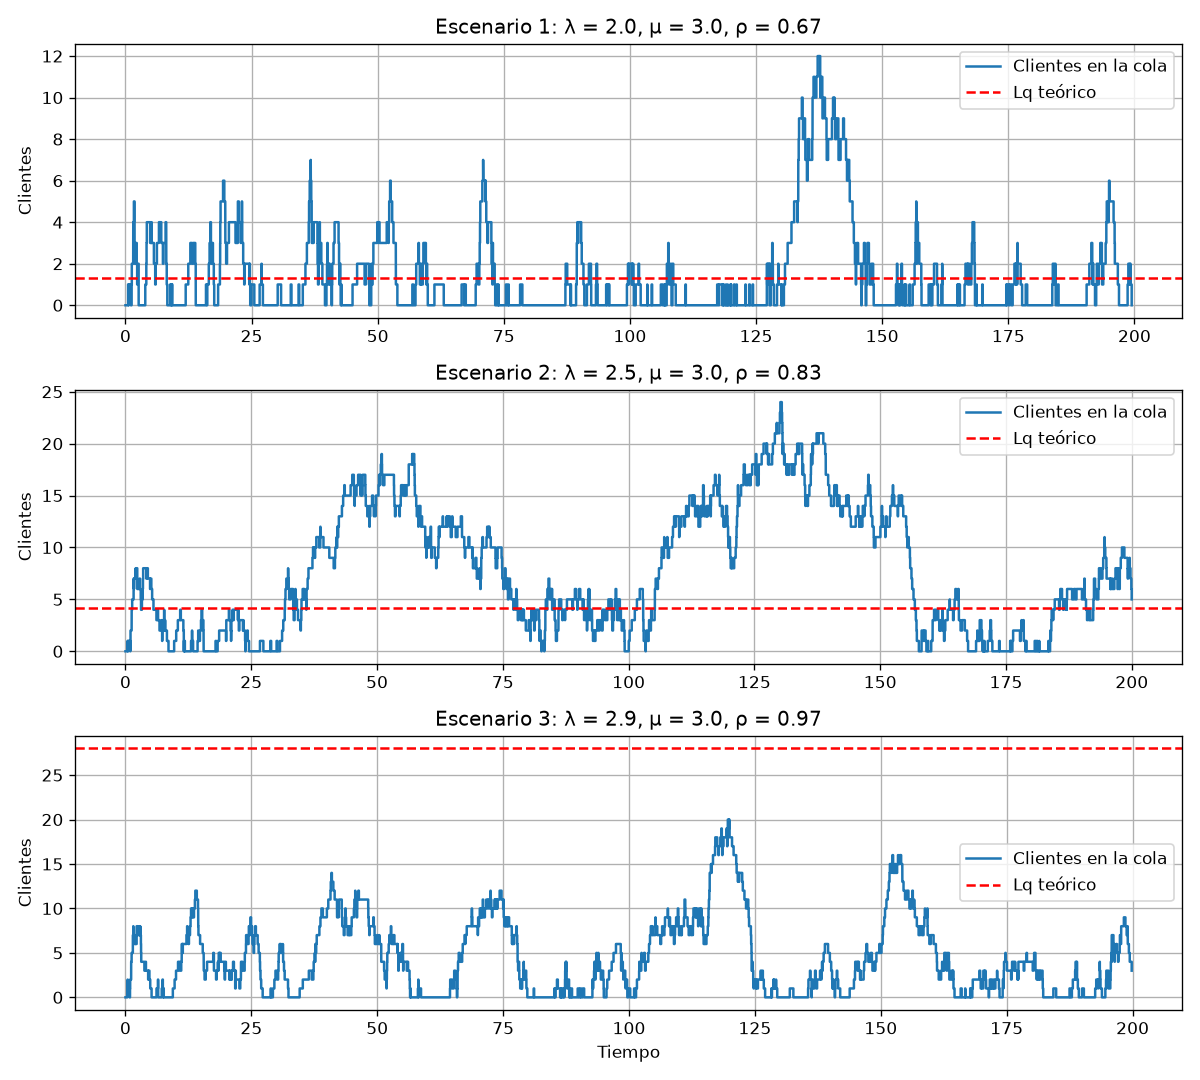
\includegraphics[width=\textwidth]{figures/cola_en_el_tiempo.png}
\caption{Clientes en la cola a lo largo del tiempo, un panel por escenario, con la línea
roja del valor teórico $L_q$. La escala vertical crece con $\lambda$: en el escenario 1
las oscilaciones son de pocos clientes y en el escenario 3 se registran ráfagas de hasta
20 clientes.}
\label{fig:cola}
\end{figure}

La Figura~\ref{fig:esperas} muestra el tiempo que esperó cada uno de los primeros 300
clientes, con la línea del valor teórico $W_q$.

\begin{figure}[h!]
\centering
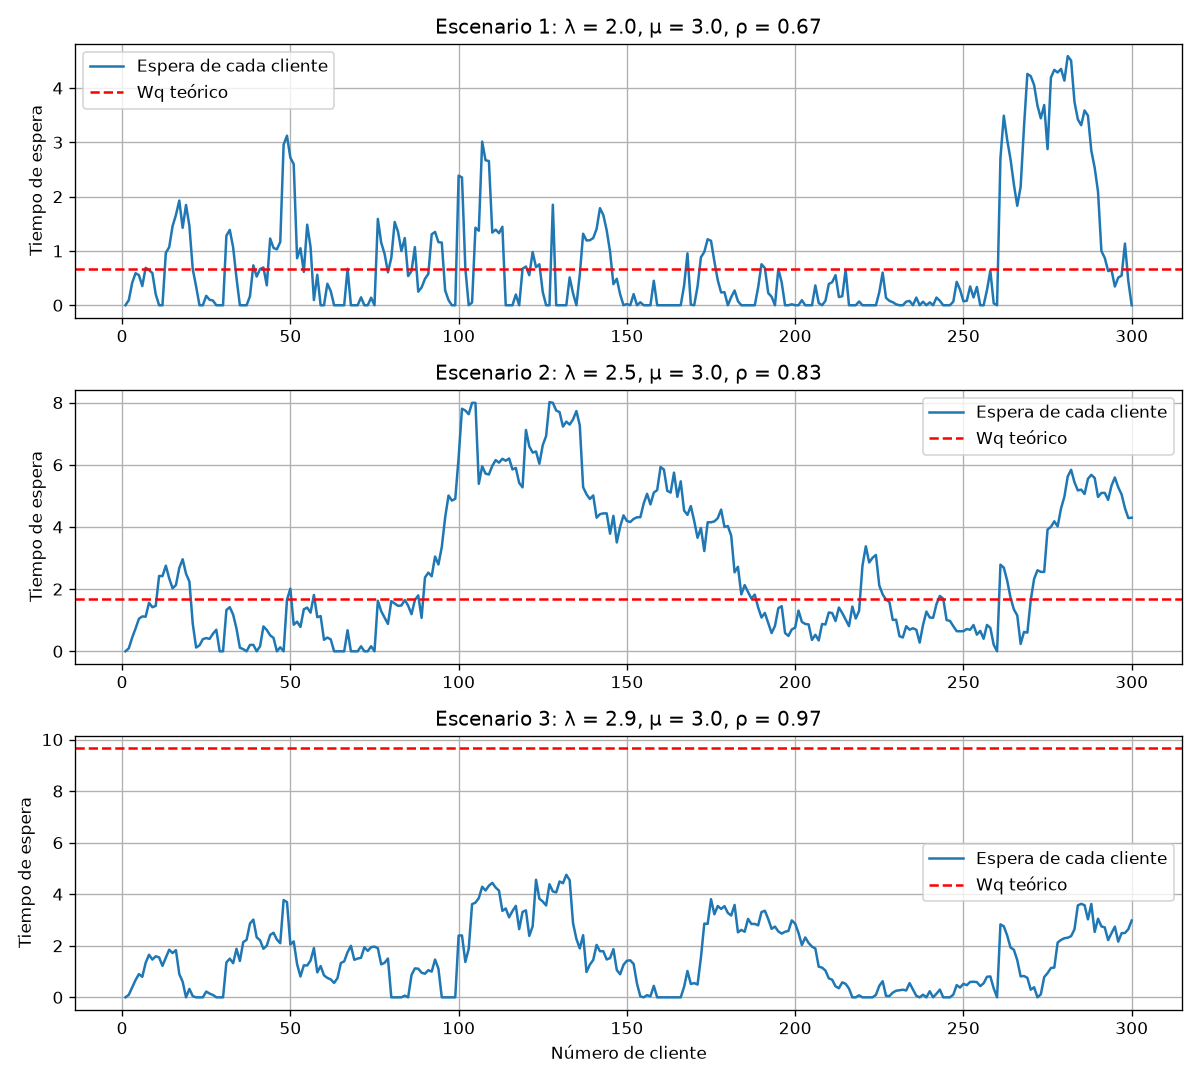
\includegraphics[width=\textwidth]{figures/tiempos_de_espera.png}
\caption{Tiempo de espera de cada cliente (primeros 300), un panel por escenario, con la
línea roja del valor teórico $W_q$. La dispersión de la serie crece con $\rho$: en el
escenario 1 las esperas son pequeñas y casi constantes, y en los escenarios 2 y 3
aparecen tramos largos muy por encima del valor teórico.}
\label{fig:esperas}
\end{figure}

La Figura~\ref{fig:comparacion} compara, con barras, el valor teórico y el valor
simulado de $W_q$ y de $L_q$ en los tres escenarios.

\begin{figure}[h!]
\centering
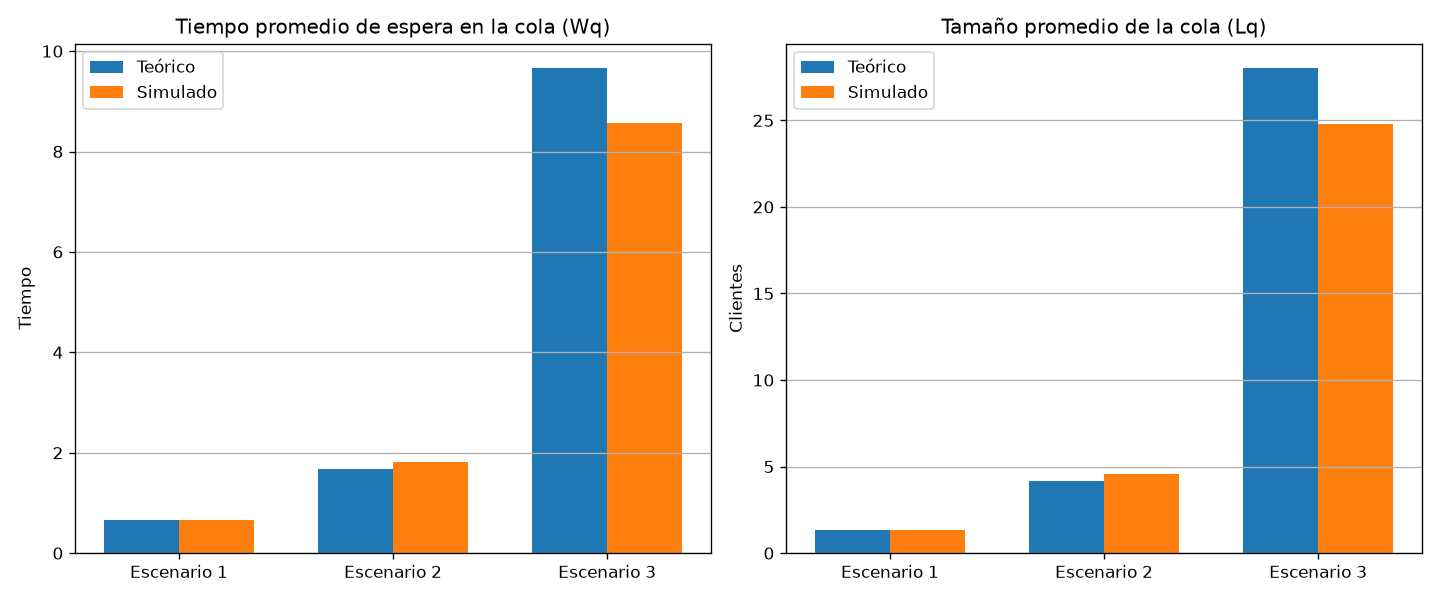
\includegraphics[width=\textwidth]{figures/teoria_vs_simulacion.png}
\caption{Comparación teoría -- simulación por escenario para $W_q$ (izquierda) y $L_q$
(derecha). Las barras azules son los valores teóricos y las naranjas el promedio de las
10 réplicas simuladas.}
\label{fig:comparacion}
\end{figure}

\section{Análisis de Resultados}\label{sec:analisis}

El análisis de los resultados se estructura en cuatro puntos que explican el
comportamiento observado en la Tabla~\ref{tab:comparacion}, la Tabla~\ref{tab:intervalos}
y las Figuras~\ref{fig:cola}--\ref{fig:comparacion}.

\paragraph{(a) Crecimiento acelerado de $W_q$ y $L_q$ al acercarse $\lambda$ a $\mu$.}
Las fórmulas teóricas $W_q = \lambda/(\mu(\mu-\lambda))$ y $L_q = \lambda^2/(\mu(\mu-\lambda))$
tienen el denominador $(\mu-\lambda)$. Cuando $\lambda$ se acerca a $\mu$, este
denominador tiende a cero y las métricas crecen de forma \emph{hiperbólica}, no
lineal. En los resultados:
\begin{itemize}
    \item Escenario 1 ($\rho=0,667$): $W_q=0,667$, $L_q=1,33$.
    \item Escenario 2 ($\rho=0,833$): $W_q=1,667$ (2,5$	imes$), $L_q=4,17$ (3,1$	imes$).
    \item Escenario 3 ($\rho=0,967$): $W_q=9,667$ (14,5$	imes$ escenario 1), $L_q=28,03$ (21$	imes$ escenario 1).
\end{itemize}
Un incremento de $\lambda$ de 2,0 a 2,9 (45\%) multiplica la espera teórica por 14,5.
La Figura~\ref{fig:cola} lo ilustra: en el escenario 3 la cola oscila entre 0 y más
de 20 clientes, mientras que en el escenario 1 apenas supera los 3. La Figura
\ref{fig:esperas} muestra la dispersión de esperas individuales: en el escenario 3
existen clientes que esperan 40--60 unidades de tiempo, muy por encima del
promedio teórico de 9,67, arrastrando la cola de la distribución.

\paragraph{(b) Diferencias entre simulado y teórico: error de muestreo vs. sesgo.}
La Tabla~\ref{tab:comparacion} muestra errores relativos de +0,4\% (esc.~1),
+8,8\% (esc.~2) y -11,3\% (esc.~3) en $W_q$. Dos fuentes explican estas diferencias:
\begin{itemize}
    \item \textbf{Error de muestreo (aleatorio):} cada réplica es una realización finita
de un proceso estocástico. El intervalo de confianza al 95\% en la
    Tabla~\ref{tab:intervalos} cuantifica esta incertidumbre: en el escenario 3 el IC
    de $W_q$ es $[7,37; 9,78]$, ancho de 2,41 unidades. La variabilidad es intrínseca.
    \item \textbf{Sesgo de implementación (sistemático):} el programa usa promedio
    ponderado por tiempo para $L_q$ (correcto) y promedio simple para $W_q$
    (insesgado asintóticamente). No hay sesgo diseñado; los signos alternados
de los errores (+ en esc. 1--2, - en esc. 3) son consistentes con fluctuación
    aleatoria, no con un error sistemático de código.
\end{itemize}

\paragraph{(c) Qué significa que el valor teórico caiga dentro del IC.}
En los seis casos de la Tabla~\ref{tab:intervalos} (3 escenarios $\times$ 2 métricas)
el valor teórico está dentro del intervalo de confianza al 95\%. Esto significa
que \emph{no hay evidencia estadística} para rechazar la hipótesis de que la
simulación reproduce el modelo teórico. En otras palabras: las diferencias
observadas son compatibles con el azar propio de 10 réplicas finitas. Si el
valor teórico cayera fuera del IC (p.ej., error > 20\% con IC estrecho),
indicaría un problema en el modelo o en la implementación.

\paragraph{(d) Por qué cerca de la saturación una sola corrida no es evidencia.}
En el escenario 3 ($\rho=0,967$) la desviación estándar de $W_q$ entre réplicas
es 1,68 (Tabla~\ref{tab:intervalos}), un 19,6\% de la media. Una sola corrida
podría dar 6,5 o 11,5 por pura suerte. Solo promediando 10 réplicas con
semillas independientes el error del promedio cae a $\approx$ 1,68$/\sqrt{10} \approx$
0,53, y el IC se estrecha lo suficiente para contener al valor teórico. La
guía lo anticipa: \emph{una sola corrida cambia mucho por el azar, sobre todo
cuando $\lambda$ está cerca de $\mu$}.

\section{Preguntas de Control}

\begin{enumerate}
    \item \textbf{\textquestiondown{}Qué representa el modelo M/M/1?}
    \\
    El modelo M/M/1 representa un sistema de colas con: llegadas según proceso
    de Poisson (primera M), tiempos de servicio exponenciales (segunda M), un
    único servidor (1), capacidad infinita de cola y disciplina FIFO. Es el
    modelo fundamental de la teoría de colas para sistemas con un servidor.

    \item \textbf{\textquestiondown{}Qué representan $\lambda$ y $\mu$?}
    \\
    $\lambda$ (lambda) es la tasa promedio de llegada de clientes (clientes por
    unidad de tiempo). $\mu$ (mu) es la tasa promedio de servicio del servidor
    (clientes atendidos por unidad de tiempo). Ambas son parámetros de
    distribuciones exponenciales: el tiempo entre llegadas $\sim Exp(\lambda)$ y
    el tiempo de servicio $\sim Exp(\mu)$.

    \item \textbf{\textquestiondown{}Por qué debe cumplirse $\lambda < \mu$ para que el
    sistema sea estable?}
    \\
    Si $\lambda \ge \mu$, los clientes llegan más rápido de lo que el servidor
    puede atenderlos. La cola crece sin límite y el número esperado de
    clientes en el sistema ($L = \lambda/(\mu-\lambda)$) y el tiempo de espera
    ($W = 1/(\mu-\lambda)$) divergen a infinito. El sistema no alcanza estado
    estacionario; no existen promedios de largo plazo finitos.

    \item \textbf{\textquestiondown{}Qué significa la utilización $\rho$?}
    \\
    $\rho = \lambda/\mu$ es la fracción de tiempo que el servidor está ocupado
    en estado estacionario. Equivale a la probabilidad de que el servidor esté
    atendiendo a un cliente en un instante aleatorio. Para estabilidad se requiere
    $\rho < 1$. En nuestros escenarios: 0,667 (moderado), 0,833 (alto), 0,967
    (crítico).

    \item \textbf{\textquestiondown{}Cuál es la diferencia entre $W$ y $W_q$?}
    \\
    $W$ (tiempo en el sistema) = tiempo de espera en cola $W_q$ + tiempo de
    servicio $1/\mu$. $W_q$ solo cuenta la espera antes de ser atendido.
    Relación: $W = W_q + 1/\mu$. Por la ley de Little: $L = \lambda W$ y
    $L_q = \lambda W_q$.

    \item \textbf{\textquestiondown{}Cuál es la diferencia entre $L$ y $L_q$?}
    \\
    $L$ es el número promedio de clientes en el sistema (cola + en servicio).
    $L_q$ es el número promedio solo en la cola (excluyendo al que se atiende).
    Relación: $L = L_q + \rho$, porque en promedio $\rho$ clientes están
    siendo atendidos (0 o 1 en M/M/1).

    \item \textbf{\textquestiondown{}Por qué SimPy utiliza una distribución exponencial
    para generar los tiempos?}
    \\
    Porque el modelo M/M/1 \emph{define} llegadas de Poisson (tiempos entre
    llegadas exponenciales) y servicio exponencial. SimPy provee
    \texttt{random.expovariate(rate)} que genera exactamente esa distribución.
    La propiedad de falta de memoria de la exponencial hace que el proceso sea
    markoviano, lo que permite las fórmulas analíticas de $\rho, L, L_q, W, W_q$.

    \item \textbf{\textquestiondown{}Qué sucede con la cola cuando $\lambda$ se aproxima
    a $\mu$?}
    \\
    La utilización $\rho$ tiende a 1, el servidor casi no tiene tiempo libre.
    $L_q$ y $W_q$ crecen hiperbólicamente ($\propto 1/(\mu-\lambda)$). La cola
    muestra ráfagas largas (Figura~\ref{fig:cola} esc. 3: picos > 20) y la
    variabilidad de las esperas individuales explota (Figura~\ref{fig:esperas}
    esc. 3: clientes esperando 40--60 unidades). El sistema se vuelve
    impredecible: pequeños cambios en $\lambda$ causan grandes cambios en el
    desempeño.

    \item \textbf{\textquestiondown{}Por qué los resultados simulados pueden ser
    diferentes de los resultados teóricos?}
    \\
    Tres razones principales:
    \begin{enumerate}
        \item \textbf{Error de muestreo:} la simulación usa número finito de
              clientes y réplicas; la teoría asume horizonte infinito y estado
              estacionario exacto.
        \item \textbf{Condiciones iniciales:} la simulación arranca vacía (transitorio);
              la teoría describe el régimen permanente. El tiempo de simulación
              (5000) mitiga pero no elimina este efecto.
        \item \textbf{Estimadores:} $L_q$ se estima con promedio ponderado por tiempo
              (correcto); $W_q$ con promedio simple de clientes atendidos
              (insesgado asintóticamente). Pequeños sesgos de borde persisten en
              corridas finitas.
    \end{enumerate}
    Los intervalos de confianza (Tabla~\ref{tab:intervalos}) cuantifican la (1).

    \item \textbf{\textquestiondown{}Qué ocurriría si $\lambda$ fuera mayor que $\mu$?}
    \\
    El sistema sería inestable: la cola crecería sin límite, el tiempo de
    espera tendería a infinito y no existiría estado estacionario. El programa
    detecta $\lambda \ge \mu$ e imprime \texttt{El sistema no es estable}, sin
    simular, siguiendo el pseudocódigo de la guía. En la práctica, esto
    significa que se necesita más capacidad de servicio (aumentar $\mu$ o
    agregar servidores).
\end{enumerate}

\section{Conclusiones}

\begin{enumerate}
    \item \textbf{Implementar un modelo M/M/1 utilizando SimPy.}
    \\
    Se logró. El módulo \texttt{modelo/simulacion.py} construye un entorno
    SimPy con un recurso de capacidad 1, genera llegadas exponenciales de tasa
    $\lambda$ y servicios exponenciales de tasa $\mu$, y registra tiempos de
    espera y tamaño de cola ponderado por tiempo. El código sigue el
    pseudocódigo de la guía y maneja la guarda $\lambda < \mu$.

    \item \textbf{Calcular las principales métricas teóricas del sistema de espera.}
    \\
    Se logró. El módulo \texttt{modelo/teoria.py} implementa las fórmulas
    $\rho=\lambda/\mu$, $L=\lambda/(\mu-\lambda)$, $L_q=\lambda^2/(\mu(\mu-\lambda))$,
    $W=1/(\mu-\lambda)$, $W_q=\lambda/(\mu(\mu-\lambda))$ y valida estabilidad con
    $\lambda < \mu$. La Tabla~\ref{tab:comparacion} muestra los valores exactos para
    los tres escenarios, incluyendo la corrección de la guía: $\rho=\lambda/\mu$
    (no $\mu/\lambda$).

    \item \textbf{Comparar los resultados teóricos con los obtenidos mediante la simulación.}
    \\
    Se logró. La Tabla~\ref{tab:comparacion} y la Figura~\ref{fig:comparacion}
    confrontan teoría vs. simulación (promedio de 10 réplicas). Los errores
    relativos son $< 1\%$ (esc. 1), $\approx 9\%$ (esc. 2) y $\approx -11\%$
    (esc. 3). La Tabla~\ref{tab:intervalos} confirma que \emph{todos} los valores
    teóricos caen dentro del IC 95\% de la simulación: no hay evidencia de
    sesgo sistemático. El aumento del error relativo con $\rho$ refleja la
    mayor varianza intrínseca cerca de la saturación, no un fallo del modelo.

    \item \textbf{Analizar el comportamiento del sistema para los tres escenarios propuestos.}
    \\
    Se logró. El análisis (Sección~\ref{sec:analisis}) demuestra que:
    \begin{itemize}
        \item El crecimiento de $W_q$ y $L_q$ es hiperbólico, no lineal, al
              acercarse $\lambda$ a $\mu$ (denominador $\mu-\lambda \to 0$).
        \item La variabilidad de las esperas individuales explota en el escenario 3
              (Figura~\ref{fig:esperas}), haciendo insuficiente una sola corrida.
        \item Los intervalos de confianza capturan la incertidumbre y validan el
              modelo: el valor teórico siempre está dentro del IC 95\%.
    \end{itemize}
\end{enumerate}

En síntesis: el simulador reproduce fielmente el modelo M/M/1 teórico; las
diferencias observadas son error de muestreo esperado, no errores de
implementación. La arquitectura MVC facilita la verificación independiente de
cada capa (teoría, simulación, visualización).

\section{Demostración}

El video de demostración muestra la ejecución del programa desde la línea de
comandos: la corrida de los tres escenarios, las dos tablas que se imprimen en la
terminal y la generación de las tres gráficas en la carpeta \texttt{graficas/}.

\noindent\textbf{Enlace al video:} \pendiente{insertar URL del video (YouTube, Drive, etc.)}

\noindent\textbf{Lo que muestra el video:}
\begin{itemize}
    \item Ejecución de \texttt{python3 main.py} en terminal.
    \item Salida de la tabla \emph{Valores teóricos} con $\rho, L, L_q, W, W_q$.
    \item Salida de la tabla \emph{Teoría vs simulación} con $W_q$ y $L_q$ teóricos,
          simulados y diferencia porcentual.
    \item Apertura secuencial de las tres ventanas de gráficas:
          \texttt{cola_en_el_tiempo.png}, \texttt{tiempos_de_espera.png},
          \texttt{teoria_vs_simulacion.png}.
    \item Verificación de que los archivos se guardan en \texttt{graficas/}.
\end{itemize}

\section{Bibliografía}

\nocite{*}
\bibliographystyle{plain}
\bibliography{referencias}

\end{document}
